%%%%%%%%%%%%%%%%%%%%%%%%%%%%%%%%%%%%%%%%%%%%%%%%%%
%	JASA LaTeX Template File
%  For use in making articles using JASAnew.cls
% July 26, 2017
%%%%%%%%%%%%%%%%%%%%%%%%%%%%%%%%%%%%%%%%%%%%%%%%%%

%% Step 1:
%% Uncomment the style that you want to use:

%%%%%%% For Preprint
%% For manuscript, 12pt, one column style

%% Comment this out if you'd rather use another style:
\documentclass[preprint]{JASAnew}

%%%%% Preprint Options %%%%%
%% The track changes option allows you to mark changes
%% and will produce a list of changes, their line number
%% and page number at the end of the article.
%\documentclass[preprint,trackchanges]{JASAnew}

%% authaffil option will make affil immediately
% follow author, otherwise authors are grouped, and affiliations
% are stacked underneath all the authors.
%\documentclass[preprint,authaffil]{JASAnew}

%% NumberedRefs is used for numbered bibliography and citations.
%% Default is Author-Year style.
%% \documentclass[preprint,NumberedRefs]{JASAnew}

%%%%%%% For Reprint
%% For appearance of finished article; 2 columns, 10 pt fonts

% \documentclass[reprint]{JASAnew}

%%%%% Reprint Options %%%%%

%% For testing to see if author has exceeded page length request, use 12pt option
%\documentclass[reprint,12pt]{JASAnew}

% authaffil option will make affil immediately
% follow author, otherwise authors are grouped, and affiliations
% are stacked underneath all the authors.
%\documentclass[reprint,authaffil]{JASAnew}

%% NumberedRefs is used for numbered bibliography and citations.
%% Default is Author-Year style.
% \documentclass[reprint,NumberedRefs]{JASAnew}

%% TurnOnLineNumbers
%% Make lines be numbered in reprint style:
% \documentclass[reprint,TurnOnLineNumbers]{JASAnew}

\usepackage{fontspec}

    \setmainfont[]{FreeSerif}

\usepackage{natbib}


\usepackage{cleveref}
\usepackage{ctable}

\begin{document}
%% the square bracket argument will send term to running head in
%% preprint, or running foot in reprint style.

\title[A subtitle goes on another line]{This is a title and this is too}

% ie
%\title[JASA/Sample JASA Article]{Sample JASA Article}

%% repeat as needed

\author{Stefano Coretta}
% ie
%\affiliation{Department1,  University1, City, State ZipCode, Country}
\affiliation{The University of Manchester}
%% for corresponding author
\email{stefano.coretta@manchester.ac.uk}
%% for additional information
\thanks{other info}

% ie
% \author{Author Four}
% \email{author.four@university.edu}
% \thanks{Also at Another University, City, State ZipCode, Country.}

%% For preprint only,
%  optional, if you want want this message to appear in upper left corner of title page
% \preprint{}

%ie
%\preprint{Author, JASA}

% optional, if desired:
%\date{\today}

\begin{abstract}
% Put your abstract here. Abstracts are limited to 200 words for
% regular articles and 100 words for Letters to the Editor. Please no
% personal pronouns, also please do not use the words ``new'' and/or
% ``novel'' in the abstract. An article usually includes an abstract, a
% concise summary of the work covered at length in the main body of the
% article.
Put your abstract here.
\end{abstract}

%% pacs numbers not used

\maketitle

%  End of title page for Preprint option --------------------------------- %

%% See preprint.tex/.pdf or reprint.tex/.pdf for many examples


%  Body of the article
\hypertarget{introduction}{%
\section{Introduction}\label{introduction}}

Almost 100 years of research have repeatedly shown that consonantal
voicing has an effect on preceding vowel duration: vowels followed by
voiced obstruents are longer than when followed by voiceless ones
\citep{heffner1937, house1953, belasco1953, peterson1960, halle1967, chen1970, klatt1973, lisker1974, raphael1975, javkin1976, maddieson1976, farnetani1986, kluender1988, laeufer1992, fowler1992, hussein1994, esposito2002, lampp2004, warren2005, durvasula2012}.
Evidence for such so called `voicing effect' has been found in a variety
of languages, including (but not limited to) English, German, Hindi,
Russian, Italian, Arabic, and Korean \citep[see][ for a more
comprehensive, but still not exhaustive list]{maddieson1976}. Despite of
the plethora of evidence in support of the \emph{existence} of the
voicing effect, still after 100 years agreement hasn't been reached
regarding the source of this effect.

Several proposal have been put forward as to where to look for the
possible cause of the voicing effect \citep[see][ and
\citet{soskuthy2013} for an overview]{maddieson1976}. Most of the
proposed accounts place the source of the voicing effect in properties
of speech
production.\footnote{Two accounts that point to perceptual features are \citet{javkin1976} and \citet{kluender1988}. To the best of my knowledge, \citet{javkin1976}'s proposal remains empirically untested, while see \citet{fowler1992} for arguments against \citet{kluender1988}.}
One of these production accounts, which will be the focus of this study,
relates the voicing effect to some constant property of speech that is
held constant across contexts while the local property of voiceless
vs.~voiced obstruents varies, thus creating a trade-off solution within
the constant property. \citet{lindblom1967}, \citet{slis1969a},
\citet{slis1969}, and \citet{lehiste1970} (among others) argue that the
relevant invariant property of speech is a constant durational interval
within which segments of different duration results in different
duration of other segments. Both the syllable/VC sequence (Lindblom) and
the word (Lehiste, Slis) has been proposed as the fixed interval. The
closure of voiced stops is shorter than that of voiceless stops. It
follows that vowels followed by shorter closures (like in the case of
voiced stops) are longer than vowels followed by longer closures (like
in the case of voiceless stops).

However, \citet{chen1970} and \citet{maddieson1976} criticise the
compensatory temporal adjustment account on empirical grounds.
\citet{chen1970} shows that the duration of the syllable is affected by
consonant voicing \citep[compatible with findings in][]{jacewicz2009},
contrary to Lindblom's expectations. \citet{maddieson1976} reject any
compensatory account based on data from a parallel of the voicing
effect, the aspiration effect, by which vowel tend to be longer when
followed by aspirated stops than when followed by non-aspirated stops.
They find no compensatory pattern between vowel and consonant duration:
the consonant /t/, which has the shortest duration, is preceded by the
shortest vowel, and vowels before /d/ and /tʰ/ have the same duration
although the durations of the two consonant are different.

\hypertarget{the-present-study}{%
\subsection{The present study}\label{the-present-study}}

An exploratory study of acoustic data from Italian and Polish was
conducted to investigate the relationship between vowel duration and
consonant voicing in two languages that reportedly differ in the
magnitude of the voicing effect. Italian has been unanimously reported
as a voicing effect language
\citep{caldognetto1979, farnetani1986, esposito2002}. The mean
difference in vowel duration when followed by voiceless vs.~voiced
consonants ranges between 22 and 24 ms \citep[with longer vowels
followed by voiced
consonants,][]{farnetani1986, esposito2002}.\footnote{These estimates should be taken as a gross approximation.
There are several issues: number of speakers, different contexts, statistical modelling.}
On the other hand, Polish is subject to conflicting results regarding
the presence and magnitude of the effect. While \citet{keating1984}
reports no effect of voicing on vowel duration in data from 24 speakers,
\citet{nowak2006} finds that vowels followed by voiced stops are 4.5 ms
longer in the 4 speakers recorded. Moreover, \citet{malisz2008} argue
based on data from 40 speakers that the magnitude of the voicing effect
in Polish is highly idiosyncratic, and claim their results to be
inconclusive.

I couldn't find evidence for a different magnitude of the effect of
voicing on vowel duration in Italian and Polish. However, the data
support a compensatory temporal adjustment account by which the
placement of the closure onset within an interval which is invariant
between voiceless and voiced contexts (which is insensitive to C2
voicing) determines the respective durations of the vowel and the stop
closure. While the data from the present study confirms that word is not
affected as shwon in \ldots{}, a problem of that account is that they
don't discuss the internal structure of the word. While it is true that
the duration of words is not affected by C2 voicing, I will show that
the interval between two consecutive releases corresponds to a more
elegant view, which is in turn compatible with current theories of
gestural timing (which fits with current views on gestural timing {[}add
references to C-centre{]}). I will show that the Release to Release is
invariant and that this is compatible with a gestural timing in which
the C2 is right-edge aligned with C1/V. I will also offer an
interpretation of \citet{maddieson1976} that is compatible with a
compensatory temporal adjustment account.

\hypertarget{method}{%
\section{Method}\label{method}}

\hypertarget{participants}{%
\subsection{Participants}\label{participants}}

Seventeen subjects in total participated to this exploratory study.
Eleven participants were native speakers of Italian (5 female, 6 male),
while six were native speakers of Polish (3 female, 3 male). The Italian
speakers were from the North and Centre of Italy (8 speakers from
Northern Italy, 3 from Central Italy). The Polish group had 2 speakers
from Poznań and 4 speakers from Eastern Poland. For more information on
the speakers, see \Cref{a:socioling}. Ethical clearance was obtained for
this study from the University of Manchester (REF 2016-0099-76). The
participants signed a written consent and received a monetary
compensation.

\hypertarget{equipment}{%
\subsection{Equipment}\label{equipment}}

The acquisition of the audio signal was achieved with the software
Articulate Assistant Advanced™ (AAA, v2.17.2) running on a
Hawlett-Packard ProBook 6750b laptop with Microsoft Windows 7, with a
sample rate of 22050 MHz (16-bit) in a proprietary format. A FocusRight
Scarlett Solo pre-amplifier and a Movo LV4-O2 Lavalier microphone were
used for audio recording.

\hypertarget{materials}{%
\subsection{Materials}\label{materials}}

The target stimuli were disyllabic words with
C\textsubscript{1}V\textsubscript{1}C\textsubscript{2}V\textsubscript{2}
structure, where C\textsubscript{1} = /p/, V\textsubscript{1} = /a, o,
u/, C\textsubscript{2} = /t, d, k, g/, and V\textsubscript{2} =
V\textsubscript{1} (e.g. /pata/, /pada/, /poto/, etc.). The lexical
stress of the target words was placed by speakers of both Italian and
Polish on V\textsubscript{1}, as intended. The make-up of the target
words was constrained by the design of the experiment, which included
ultrasound tongue imaging (UTI). Front vowels are difficult to image
with UTI, since their articulation involves tongue positions which are
particularly far from the ultrasonic probe, hence reducing the
visibility of the tongue contour. For this reason, only central and back
vowels were included. Since one of the variables of interest in the
exploratory study was the closing gesture of C\textsubscript{2}, only
lingual consonants were used. A labial stop was chosen as the first
consonant to reduce possible coarticulation with the following vowel
(although see \citealt{vazquez-alvarez2007}). The target words were
embedded in a frame sentence, \emph{Dico X lentamente} `I say X slowly'
in Italian \citep[following][]{hajek2008}, and \emph{Mówię X teraz} `I
say X now' in Polish. These sentences were chosen in order to keep the
placement of stress and emphasis similar across languages, so to ensure
comparability of results.

\hypertarget{procedure}{%
\subsection{Procedure}\label{procedure}}

The participant was asked to read the sentences with the target words
which were sequentially presented on the computer screen. The order of
the sentence stimuli was randomised for each participant. Each
participant read the list of randomised sentence stimuli six times. Due
to software constraints, the order of the list was kept the same across
the six repetitions within each participant. Each speaker read a total
of 72 sentences, with a grand total of 576 tokens (288 per language).
The reading task lasted between 15 and 20 minutes, with optional short
breaks between one repetition and the other.

\hypertarget{data-processing-and-measurements}{%
\subsection{Data processing and
measurements}\label{data-processing-and-measurements}}

\ctable[caption = List of measurements as extracted from acoustics.,
label = t:dur-measures,
width=\textwidth,
star
]{ll>{\raggedright}p{9cm}}{}{
\FL
\textbf{landmark}               &                  & \textbf{criteria}                                                                                    \ML
vowel onset           & (V1 onset)         & appearance of higher formants in the spectrogram following the burst of /p/ (C1)            \NN
vowel offset          & (V1 offset)        & disappearance of the higher formants in the spectrogram preceding the target consonant (C2) \NN
consonant onset       & (C2 onset)         & corresponds to V1 offset                                                                    \NN
closure onset         & (C2 closure onset) & corresponds to V1 offset                                                                    \NN
consonant offset      & (C2 offset)        & appearance of higher formants of the vowel following C2 (V2); corresponds to V2 onset                                \NN
consonant release & (C1/C2 release)         & automatic detection + manual correction \citep{ananthapadmanabha2014}                                           \LL
}

The audio recordings were exported from AAA in \texttt{.wav} format for
further processing. A forced aligned transcription was accomplished
through the SPeech Phonetisation Alignment and Syllabification software
(SPPAS) \citep{bigi2015}. The outcome of the automatic annotation was
manually corrected when necessary, according to the criteria in
\Cref{t:dur-measures}. The releases of C1 and C2 were detected
automatically by means of a Praat scripting implementation of the
algorithm described in \citet{ananthapadmanabha2014}. The durations in
milliseconds of the following intervals were extracted from the
annotated acoustic landmarks with Praat scripting: sentence duration,
word duration, vowel duration (V1 onset to V1 offset), consonant closure
duration (V1 offset to C2 burst), and Release-to-Release duration (RR
duration, C1 release to C2 release). Syllable rate (syllables per
second) was used as a proxy to speech rate \citep{plug2018} for duration
normalisation, and was calculated as the number of syllables divided by
the duration of the sentence (8 syllables in Italian, 6 in Polish).

\hypertarget{statistical-analysis}{%
\subsection{Statistical analysis}\label{statistical-analysis}}

Given the exploratory nature of the study, all statistical analyses
reported here are to be considered data-driven or hypothesis-generating
rather than hypothesis-driven \citep{kerr1998}. The durational
measurements were analysed with linear mixed-effects models using
\texttt{lme4} v1.1-17 in R v3.5.0 \citep{r-core-team2018, bates2015}.
All factors were coded with treatment contrasts. \emph{P}-values for the
individual terms were obtained with \texttt{lmerTest} v3.0-1, which uses
the Satterthwaite's approximation to degrees of freedom
\citep{kuznetsova2017}. \emph{P}-values below the alpha level 0.05 were
considered significant. The estimates of the relevant effects are then
calculated by refitting the models including only the significant terms
\citep[step-down approach,][pp.~121--122]{diggle2002, zuur2009}. Bayes
factors were used to specifically test the null hypotheses that word and
RR duration are not affected by C2 voicing (i.e., the effect of C2
voicing on duration is \texttt{0}). For each set of null/alternative
hypotheses, a full model (with the predictor of interest) and a null
model (excluding it) were fitted separately using Maximum Likelihood
estimation \citep[p.~34]{bates2015}. The BIC approximation was then used
to obtain Bayes factors
\citep{raftery1995, raftery1999, wagenmakers2007, jarosz2014}. The
approximation is calculated according to the equation in \ref{eq:bayes}
\citep[p.~796]{wagenmakers2007}.

\begin{equation}
\label{eq:bayes}
BF_{01} \approx exp(\Delta{}BIC_{10}/2)
\end{equation}

where \(\Delta{}BIC_{10} = BIC_1 - BIC_0\), \(BIC_1\) is the BIC of the
full model, and \(BIC_0\) is the BIC of the null model. Values of
\(BF_{01} > 1\) indicate a preference of H\textsubscript{0} over
H\textsubscript{1}. The interpretation of the Bayes factors follows the
recommendations in \citet[p.~139]{raftery1995}.

\hypertarget{results}{%
\section{Results}\label{results}}

Only the most relevant terms will be presented. For the others see
tables and appendixes.

\hypertarget{vowel-duration}{%
\subsection{Vowel duration}\label{vowel-duration}}

A linear mixed-effects model was fitted with the following terms: vowel
duration as the outcome variable; fixed effects for C2 voicing
(voiceless, voiced), vowel (a, o, u), language (Italian, Polish), and
speech rate (as syllables per second); by-speaker and by-word random
intercept with by-speaker random slopes for C2 voicing. All possible
interactions between C2 voicing, vowel, and language were included. The
following terms are significant: C2 voicing, vowel, language, and speech
rate. No interaction was significant. The vowel /a/ (when followed by
voiceless stops) has a duration of 202.5 ms (se = 8.5 ms). The vowel /o/
is 9.5 ms shorter (se = 3 ms), while the vowel /u/ is 30.5 ms shorter
(se = 3). Vowels are 11 ms longer (se = 3) when followed by a voiced
stop. Polish has on average shorter vowels than Italian (\(\hat{\beta}\)
= -28 ms, se = 8 ms), although the effect of voicing is estimated to be
the same in both languages (the interaction of language and C2 voicing
is not significant). Speech rate has a negative effect on vowel
duration, such that faster rates correlate with shorter vowel durations
(\(\hat{\beta}\) = -15 ms, se = 1 ms).

\hypertarget{consonant-closure-duration}{%
\subsection{Consonant closure
duration}\label{consonant-closure-duration}}

The same maximally specified model as with vowel duration has been
fitted to consonant closure durations as the outcome variable. Only C2
voicing and speech rate were significant. Stop closure is 13 ms shorter
(se = 3 ms) if the stop is voiced. Finally, faster speech rates
correlate with shorter closure durations (\(\hat{\beta}\) = -8 ms, se =
1 ms).

\hypertarget{vowel-and-closure-duration}{%
\subsection{Vowel and closure
duration}\label{vowel-and-closure-duration}}

The full model was specified with the following terms and interactions:
vowel duration as the outcome variable; as fixed effects, closure
duration, vowel, speech rate; an interaction between closure duration
and vowel; by-speaker and by-word random intercepts, and by-speaker
random slopes for C2 voicing. Closure duration has a significant effect
on vowel duration when the vowel is /a/ (\(\hat{\beta}\) = -0.2 ms, se =
0.06 ms). The effect with the vowel /o/ does not significantly differ
from the one with /a/, while with /u/ the effect is -0.5 ms
(\(\hat{\beta}\) = -0.3 ms, se = 0.06 ms). In general, then, closure
duration is inversely correlated with vowel duration after controlling
for speech rate. However the correlation is quite weak. A 1 ms increase
in closure duration corresponds to a 0.2--0.5 ms decrease in vowel
duration.

\hypertarget{word-duration}{%
\subsection{Word duration}\label{word-duration}}

The following full and null models were fitted to test whether word
duration is affected by C2 voicing. In the full model, I entered as
fixed effects: C2 voicing, C2 place, vowel, speech rate, and language.
The model also included by-speaker and by-word random intercepts, plus a
by-speaker random slope for C2 voicing. The null model was the same as
the full model, with the exclusion of the fixed effect of C2 voicing.
The Bayes factor of the null model against the full model is 21.5. Thus,
the null model (in which the effect of C2 voicing is 0) is 21.5 times
more likely under the observed data than the full model. This indicates
that there is strong evidence for word duration not being affected by C2
voicing.

\hypertarget{release-to-release-interval-rr-duration}{%
\subsection{Release to Release interval (RR)
duration}\label{release-to-release-interval-rr-duration}}

The models specifications for the RR duration were the same as for word
duration. The Bayes factor of the null model against the full model for
RR duration is 19, which means that the null model (without C2 voicing)
is 19 times more likely than the full model. The data suggests there is
positive evidence that duration of the RR interval is not affected by C2
voicing.

\hypertarget{discussion}{%
\section{Discussion}\label{discussion}}

In this exploratory study of Italian and Polish acoustic data, I found
that the duration of interval between the releases of two consecutive
consonants is insensitive to the phonological voicing of the second
consonant. The difference in vowel duration before voiceless vs.~voiced
stops derives from differences in placement of the closure onset within
the fixed interval between the releases of C1 and C2.

\hypertarget{gestural-alignment}{%
\subsection{Gestural alignment}\label{gestural-alignment}}

\label{s:gestural}

\begin{figure}
  \centering
  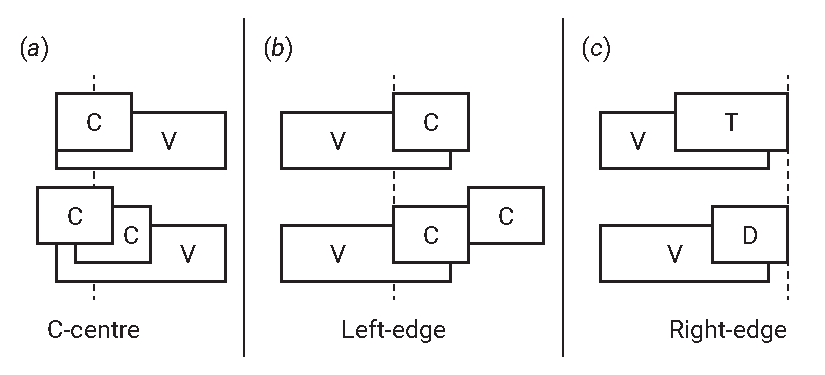
\includegraphics{img/gorganisation.pdf}
  \caption{Gestural organisation patterns for onsets (a), codas (b), heterosyllabic onsets (c). See \Cref{s:gestural} for details. Based on \citet{marin2010}.}
  \label{f:gorganisation}
\end{figure}

According to the coupled oscillator model of syllabic structure (ref
\ldots{}), articulatory gestures can be timed according to two coupling
modes: in-phase (synchronous) mode, by which two gestures start in
synchrony, or anti-phase (sequential) mode, in which one gesture starts
when the preceding gesture has reached its target. \citet{marin2010}
showed that onset consonants in American English are in-phase with the
vowel nucleus and anti-phase with each other in the case of onset
clusters. Such phasing pattern establishes a stable relation between the
centre of the consonant or consonant cluster and the following vowel.
Independent of the number of onset consonants, the midpoint of the
onset, the so-called `C-centre', is maintained at a fixed distance from
the vowel, such that increasing number of consonants in the onset does
not change the C-center/vowel distance. On the other hand, coda
consonants are timed anti-phase with the preceding vowel and between
themselves. Stability in codas is seen in the lag between the vowel and
the left-most edge of the coda, which is not affected by the number of
coda consonants. Other studies found further evidence for the
synchronous and sequential coupling modes (ref from Marin 2014),
although which of the two modes is used depends on the language and the
consonants under study.

Consonants can thus be said to follow either a C-centre organisation
pattern or a left-edge organisation pattern. In both cases, of course,
the pattern is relative to the tautosyllabic vowel (the following vowel
for onsets, the preceding vowel for codas). To the best of my knowledge,
no study has reported the timing of onset consonants relative to the
\emph{preceding} (heterosyllabic) consonant. The results from this
acoustic study on Italian and Polish are compatible with a right-edge
organisation pattern for onset consonants and preceding stressed vowels.
The release of C2 (which is the onset of the seconds in CVCV words),
which can be thought as the acoustic parallel of the articulatory right
edge of C2, is invariantly timed relative to V1 (which is the nucleus of
the first syllable).

A consequence of a right-edge organisation pattern is that differences
in C2 closure duration do not affect the lag between V1 and the release
of C2, as shown by the results of this study. The invariance of the lag
between the release of C1 and that of C2 then can be seen to follow from
the invariance in timing between, on the one hand, C1 (which is always
/p/ in this study) and V1, and, on the other, between V1 and the right
edge of C2.

A right-edge organisation account is compatible with findings by
\citet{raphael1975}, \citet{de-jong1991}, and \citet{celata2018}.
\citet{celata2018} show that vowels before tautosyllabic clusters have
the same duration as before heterosyllabic clusters. However, vowels
followed by geminates are shorter than when followed by singletons,
although from a syllabic structure geminates correspond to
heterosyllabic clusters and singletons to tautosyllabic clusters (i.e.,
V-final syllables followed by singletons and tautosyllabic clusters are
open, while those followed by geminates and heterosyllabic clusters are
closed). \citet{celata2018} argue that these results corroborate a
rhythmic account in which the relevant unit is the rhythmic syllable,
i.e.~the VC(C) sequence (independent of the traditional syllabic
structure), which is kept constant. Such view reflects a gestural timing
view in which the timing of the right edge of the consonant is held
constant relative to the vowel.

\citet{de-jong1991} reports that the closing gesture of consonants
following stressed vowels is quicker in voiceless consonants than in
voiced ones, and that also it is timed earlier than that of voiced
consonants. The difference in vowel duration are, according to
\citet{de-jong1991}, driven by the timing of the consonantal closing
gesture relative to the vocalic opening gesture. The view proposed above
reflects these findings. Moreover, the data in \citet{de-jong1991} show
that the final portion of the vocalic opening gesture is prolonged
before voiced stops. This finding corresponds to what
\citet{raphael1975} reported based on electromyographic data. The
electromyographic signal corresponding to the vocalic gesture reaches
its plateaux at the same time in the voiceless and voiced context, but
the plateaux is held for longer in the case of vowels followed by voiced
stops, indicating that muscular activation is kept for longer.

All of these studies taken together, plus the results from this study,
bring evidence to the view that two factors contribute to the difference
in vowel duration observed before consonants varying in their voicing
specification. These two factors are (1) the right-edge alignment of
coda consonants following stressed vowels relative to the latter, and
(2) the differential timing of the closing gesture for voiceless
vs.~voiced stops. These two factors together can be synthesised into a
compensatory temporal adjustment account, in which the fixed interval is
generated by factor (1) and the temporal adjustment is brought about by
factor (2).

\hypertarget{limitations}{%
\subsection{Limitations}\label{limitations}}

It is difficult given the present data to disambiguate between two
interpretations: either C2 is timed relative to a gestural epoch of V1
(possibly the gesture onset)---and the invariance of RR would follow
from the fact that C1 is held constant--- or the motor plan for CVCV
words is structured is such a way to directly keep the RR duration
invariant.

\hypertarget{a-reinterpretation-of-maddieson1976}{%
\subsection{\texorpdfstring{A reinterpretation of
\citet{maddieson1976}}{A reinterpretation of @maddieson1976}}\label{a-reinterpretation-of-maddieson1976}}

Before concluding/Finally, I would like to offer a reinterpretation of
the results in \citet{maddieson1976}. A major drawback of the analysis
in \citet{maddieson1976} is that the consonant duration in fact was
measured from the closure of the relevant consonant to the release of
the following consonant, due to difficulties in detecting the release of
the consonant of interest (e.g., in \emph{ab sāth kaho}, the duration of
/tʰ/ in \emph{sāth} was calculated as the interval between the closure
of /tʰ/ and the release of /k/). This measure includes the burst and
(eventual) aspiration of the consonant. \citet{slis1969a}, however,
states that the inverse correlation between vowel duration and the
following consonant raises when consonant \emph{closure} duration is
taken into account, and not entire \emph{consonant} duration. If the
correlation exists between vowel and closure duration, the inclusion of
burst/aspiration duration clearly alters this relationship.

\begin{acknowledgments}
Thanks to...
\end{acknowledgments}

\appendix

\section{Socio-linguistic information of participants}
\label{a:socioling}

\ctable[caption = Participants' sociolinguistic information.,
label = t:socio,
width=\textwidth,
star,
doinside = \footnotesize
]{llll>{\raggedright}p{5cm}lll}{}{
\FL
ID & Age & Sex    & Native L & Other Ls& City of birth & Spent most time in & > 6 mo \ML
it01 & 29 & Male   & Italian & English, Spanish                          & Verbania            & Verbania        & Yes \NN
it02 & 26 & Male   & Italian & Friulian, English, Ladin-Venetan          & Udine               & Tricesimo & Yes \NN
it03 & 28 & Female & Italian & English, German                           & Verbania            & Verbania        & No  \NN
it04 & 54 & Female & Italian & Calabrese                                 & Verbania            & Verbania        & No  \NN
it05 & 28 & Female & Italian & English                                   & Verbania            & Verbania        & No  \NN
it07 & 29 & Male   & Italian & English                                   & Tradate             & Cairate         & No  \NN
it09 & 35 & Female & Italian & English                                   & Vignola & Vignola         & Yes \NN
it11 & 24 & Male   & Italian & English                                   & Monza               & Monza           & Yes \NN
it13 & 20 & Female & Italian & English, French, Arabic, Farsi            & Ancona              & Chiaravalle     & Yes \NN
it14 & 32 & Male & Italian & English, Spanish & Frosinone & Frosinone & Yes \NN
pl02 & 32 & Female & Polish  & English, Norwegian, French, German, Dutch & Koło                & Poznań          & Yes \NN
pl03 & 26 & Male   & Polish  & Russian, English, French, German          & Nowa Sol            & Poznań          & Yes \NN
pl04 & 34 & Female & Polish  & Spanish, English, French                  & Warsaw              & Warsaw          & No  \NN
pl05 & 42 & Male   & Polish  & English, French                           & Przasnysz           & Warsaw        & No  \NN
pl06 & 33 & Male   & Polish  & English                                   & Zgierz              & Zgierz          & Yes \NN
pl07 & 32 & Female & Polish  & English, Russian                          & Bielsk Podlaski     & Bielsk Podlaski & Yes \LL
}

%% before appendix (optional) and bibliography:
% \begin{acknowledgments}
%This research was supported by  ...
% \end{acknowledgments}

% -------------------------------------------------------------------------------------------------------------------
%   Appendix  (optional)

%\appendix
%\section{Appendix title}

%If only one appendix, please use
%\appendix*
%\section{Appendix title}


%=======================================================
%IMPORTANT

%Use \bibliography{<name of your .bib file>}+
%to make your bibliography with BibTeX.

%Once you have used BibTeX you
%should open the resulting .bbl file and cut and paste the entire contents
%into the end of your article.
%=======================================================

\bibliography{linguistics.bib}


\end{document}
